% Time-stamp: <09/10/02 01:57:13 vilhuber>
% $Id: Presentation-PSD.tex 396 2013-11-03 22:29:27Z lv39 $

% normal line:
\documentclass[xcolor=table,compress]{beamer}
% to create notes:
%\documentclass[handout,notes=only]{beamer}
% to create handouts
%\documentclass[xcolor=table,handout,compress]{beamer}
% to create a different kind of handouts
%\documentclass{article}
%\usepackage[envcountsect]{beamerarticle}

%\setbeameroption{handout}
%\setbeameroption{show notes}


%
% Packages
%
\mode<article> % only for the article version
{
  \usepackage{fullpage}
  \usepackage{hyperref}
}
\usepackage{ifpdf}
\ifpdf
\usepackage{embedfile}
\embedfile{\jobname.tex}
\fi

\usepackage{graphicx}
%\usepackage{pstricks}
\usepackage{xcolor}
\usepackage{pifont}
%\usepackage{../chicago}
\usepackage{pgf}
\usepackage{amsmath,amssymb,amsfonts}
\usepackage[latin1]{inputenc}
\usepackage{colortbl}
\usepackage[english]{babel}
\usepackage{array}
\usepackage{pdfpages}
% usage:
%   \includepdf[pages={1}]{myfile.pdf}
%   \includepdf[pages={1,3,5}]{myfile.pdf} would include pages 1, 3, and 5 of the file. 
%   To include the entire file, you specify pages={-}, where {-}
%\usepackage{landscape}

%\usepackage{lmodern}
%\usepackage[T1]{fontenc}

\usepackage{times}
%\usepackage{colortbl}

%============================================================
% Beamer specific styles and configs
%============================================================

\mode<presentation>
{
% alternative, could always use
%\usetheme{Census}
\usetheme{cornell}
\useoutertheme{cornell}
}


%\setbeamercovered{dynamic}


%============================================================
% Title
%============================================================

\title[Archiving and Curation]{A Proposed Solution to the Archiving and Curation of Confidential Scientific Inputs}
\author[Abowd, Vilhuber,Block]{%
  John M. Abowd\inst{1} \and
  Lars~Vilhuber\inst{1} 
\and William~Block\inst{2}%
}

\institute[Cornell]{
  \inst{1}%
   Labor Dynamics Institute,
  ILR,
\and \inst{2} Cornell Institute for Social and Economic Research,
\and 
\includegraphics[height=10pt]{cu_logo_only}  Cornell University, Ithaca, NY, USA}%
\date[September 2012]{September 2012,  PSD 2012}
\subject{Data Archive; Data Curation; Statistical Disclosure Limitation; Privacy-preserving Datamining}

%
% Some useful commands
%

\newcommand{\rarrow}{\selectfont\ding{220}}
\newcommand{\skiplink}{\tiny{\gray\selectfont\ding{59}}}
\newcommand{\goback}{\Acrobatmenu{GoBack}{\gray\selectfont\ding{242}}}
\newcommand{\x}{\selectfont\ding{52}}
\newcommand{\verbatimsize}{\tiny}
\newcommand{\tablesize}{\footnotesize}

\newenvironment{slide}{\begin{frame}}{\end{frame}}
%
% The document proper
%
\begin{document}

\frame{\titlepage}

%\part<presentation>*{Outline}
%
%\begin{frame}
%  \frametitle{Outline}
%  \tableofcontents[part=1,pausesections]
%\end{frame}

% This puts the partial table of contents at the start of each subsection
%\AtBeginSubsection[]
%{
%  \begin{frame}<beamer>
%    \frametitle{Outline}
%    \tableofcontents[current,currentsubsection]
%  \end{frame}
%}

\part<presentation>{Main Talk}

%
%  From this point on, we should probably extract it to a sub-document
%

%TCIDATA{Version=5.00.0.2570}
%TCIDATA{LaTeXparent=0,0,Presentation-CAFE-displacement-subdoc.tex}
% $Id: Presentation-PSD-subdoc.tex 396 2013-11-03 22:29:27Z lv39 $
% $URL: https://forge.cornell.edu/svn/repos/ncrn-cornell/branches/papers/PSD2012/Presentation/Presentation-PSD-subdoc.tex $

%
%
%
\section[Motivation]{Some facts that motivated us}

\begin{frame}
\frametitle{}
\begin{block}{Motivation}

\end{block}
\end{frame}

\begin{frame}
\frametitle{Replicating of research results}
\begin{block}{Critical element of science}
\begin{itemize}
\item Replication of methods, data inputs, computational environment is a critical element of the scientific approach
\item Journals, funding agencies (in the U.S.) have been moving to making archiving of inputs to scientific results more robust, even mandatory
\end{itemize}
\end{block}
\end{frame}

\begin{frame}
\frametitle{Not a new problem}
\begin{block}{Econometrica}
``In its first issue, the editor of Econometrica (1933), Ragnar Frisch, noted
the importance of publishing data such that readers could fully explore
empirical results.  Publication of data, however, was discontinued early in
the journal's history.  [...]  The journal arrived full-circle in late 2004 when Econometrica
adopted one of the more stringent policies on availability of data and
programs.
\end{block}
\tiny \href{http://www.econometricsociety.org/submissions.asp\#4}{http://www.econometricsociety.org/submissions.asp\#4} as cited in \href{http://research.stlouisfed.org/wp/2005/2005-014.pdf}{Anderson et al (2005)}
\end{frame}

\begin{frame}
\frametitle{Problem will become worse}
\begin{block}{Increased use of restricted-access data}
\begin{itemize}
\item Today's young scholars pursue research
programs that mandate inherently identifiable data
\begin{itemize}
\item Geospatial relations,
\item Exact genome data,
\item Networks of all sorts,
\item Linked administrative records
\end{itemize}
\item These researchers acquire authorized, generally unfettered, restricted access to the
confidential, identifiable data and perform their analyses in secure
environments.
\item Archiving (curation) of input data is complicated
\item Knowledge discovery is complicated
\end{itemize}
\end{block}
\end{frame}
\begin{frame}
\frametitle{Decline in the use of classic public-use data}
%\includepdf[pages={1-2}]{Chetty-1-2-Slides.pdf}
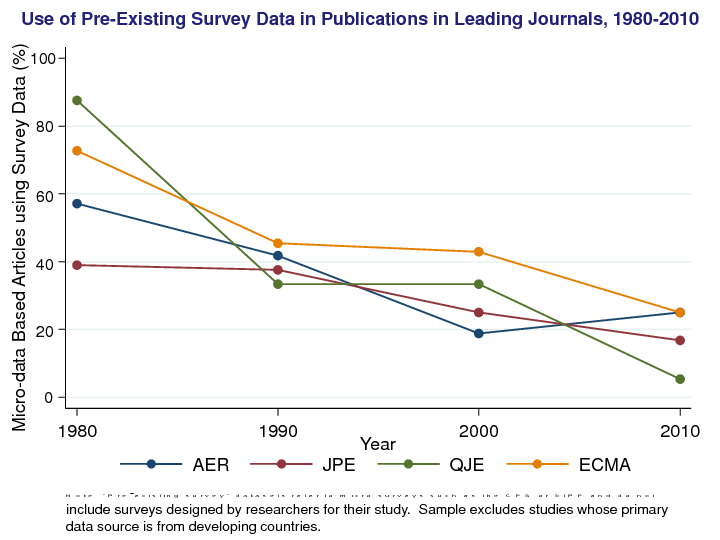
\includegraphics[width=0.8\paperwidth]{ChettySlide1}
\end{frame}

\begin{frame}
\frametitle{Increase in the use of administrative data in economics}
%\includepdf[pages={1-2}]{Chetty-1-2-Slides.pdf}
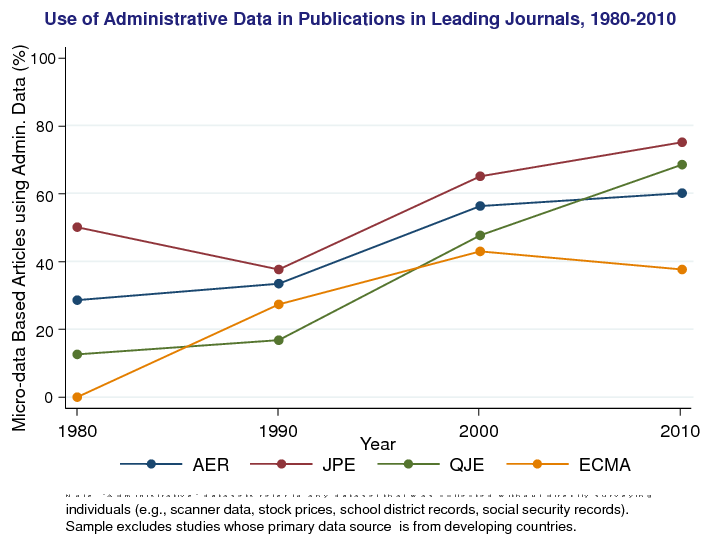
\includegraphics[width=0.8\paperwidth]{ChettySlide2}
\end{frame}

\begin{frame}
\frametitle{Not limited to economics}
\begin{block}{Nature, 2012}
``Many of the emerging `big data' applications come from private sources that are inaccessible to other researchers. The data source may be hidden, compounding problems of verification, as well as concerns about the generality of the results.''\\
\end{block}
\tiny (Huberman, Nature 482, 308 (16 February 2012) \href{http://dx.doi.org/10.1038/482308d}{doi:10.1038/482308d})
\end{frame}

\section[Problem]{Stating the problem in the U.S. case}
\begin{frame}
\frametitle{}
\begin{block}{Stating the problem}

\end{block}
\end{frame}

\begin{frame}
\frametitle{Why we think there is a problem}
\begin{block}{Core issues}
\begin{itemize}
\item[a] Insufficient curation (starting with archiving)
\item[b] No way to reference data (unique identifiers)
\item[c] No consistent way to learn about the data (metadata dissemination)
\end{itemize}
\end{block}
\end{frame}

\begin{frame}
\frametitle{Dataset usage in Census RDC}
\begin{block}{1,505 project-dataset pairs}
\centering
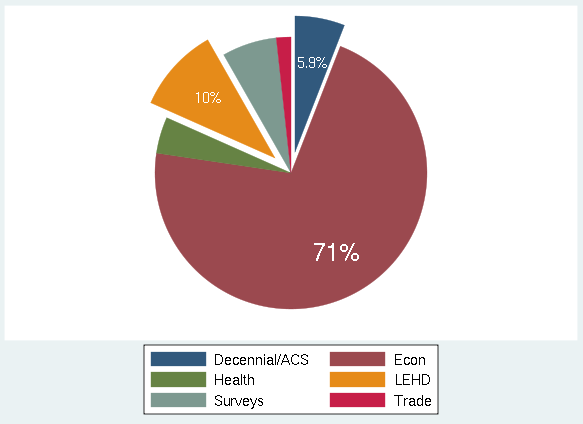
\includegraphics[width=0.8\textwidth]{../pie-chart-rdc-data}
\end{block}
\tiny Many projects use multiple datasets.
\end{frame}

\begin{frame}
\frametitle{Economic (business) datasets}
\begin{itemize}
\item 71\% of datasets are business (economic) datasets
\item Primarily establishment-based records from the
Economic Censuses and Surveys, the Business Register, and the Longitudinal Business Database (LBD)
\item They form the core of the modern
industrial organization studies \cite%
{DunneRobertsSamuelson1989,OlleyPakes1996} as well as modern gross job
creation and destruction in macroeconomics \cite%
{DavisHaltiwangerSchuh,HaltiwangerJarminMiranda2010}.
\item But there are no public-use micro-data for these establishment-based products
\item Exception: recently-released Synthetic LBD \cite%
{AbowdVilhuber2010,KinneyEtAl2011}
\item Currently no active curation (of derived datasets) [a], no way to reference [b], convoluted way to learn about the data structure [c$^*$]
\end{itemize}
\end{frame}

\begin{frame}
\frametitle{LEHD data}
\begin{block}{Linked employer-employee data}
\begin{itemize}
\item Longitudinal and cross-sectional detail
\item New confidentiality protection methodologies \cite{AbowdEtAl2012,Ashwin2008}
have unlocked large amounts of data for public-use: highly detailed local area tabulations
exist based on the {LEHD} data
\item But: no public-use micro-data exist for this
longitudinal job frame or any of its derivative files.
\item Confidential data are dynamic (quarterly changes)
\item Currently some active curation (archiving, 10-yr!) [a$^*$], no way to reference (publicly) [b$^*$], convoluted way to learn about the data structure [c$^*$]
\end{itemize}
\end{block}
\end{frame}

\begin{frame}
\frametitle{Not unique to Census Bureau}
\begin{block}{Internal Revenue Service/ Social Security Administration}
\begin{itemize}
\item
New projects (Chetty et al, 2012; von Wachter and co-authors) have created and/or used linked longitudinal data at the IRS or the Social Security Administration.
\item Neither agency has long-run experience at the statistical data curation function [a], (meta)data dissemination [b,c].
\item Although both IRS and SSA have produced statistical tables for a long time.
\end{itemize}
\end{block}
\end{frame}

\begin{frame}
\frametitle{Not unique to Census Bureau}
\begin{block}{Bureau of Labor Statistics}
\begin{itemize}
\item Long history of making time-series available
\item Limited access to microdata at the BLS 
\item Unknown curation [a]
\item Even for public-use data, no way to reference specific releases [b]
\item No well-established way to learn about microdata [c]
\end{itemize}
\end{block}
\end{frame}

\begin{frame}
\frametitle{Core problems}
\begin{columns}
  \begin{column}{0.3\textwidth}
    \begin{itemize}[<+->]
\item Curation\newline
\item Identification\newline
\item Information dissemination
    \end{itemize}
  \end{column}
  \begin{column}{0.25\textwidth}
  \begin{itemize}
  \item[\ ]\onslide<4-6>{$\leftarrow$}\newline
  \item[\ ]\onslide<5-6>{$\leftarrow$}\newline
  \item[\ ]\onslide<6>{$\leftarrow$}\newline
  \end{itemize}
  \end{column}
  \begin{column}{0.4\textwidth}
     \begin{itemize}[<+->]
        \item require cooperation of NSI
        \item partial solution (DOI)\newline
        \item core proposal\newline
     \end{itemize}
  \end{column}
\end{columns}
\end{frame}


\section[Solution]{A proposed solution}
\begin{frame}
\frametitle{}
\begin{block}{A proposed solution}

\end{block}
\end{frame}

\begin{frame}
\frametitle{Proposed solution}
\begin{block}{Core}
We develop the core of a method for solving the data archive
and curation problem that confronts the custodians of restricted-access
research data and the scientific users of such data. Our solution recognizes 
the dual protections afforded by physical security and access limitation protocols.
\end{block}
\end{frame}

\begin{frame}
\frametitle{Requirements}
\begin{block}{Royal Society (2012)}
\begin{itemize}
\item Accessible (a researcher can easily find it);
\item Intelligible (to various audiences);
\item Assessable (are researchers able make judgements about or
assess the quality of the data);
\item Usable (at minimum, by other scientists).
\end{itemize}
\end{block}
\end{frame}


\begin{frame}
\frametitle{Proposed solution}
\begin{block}{Extensible framework}
\begin{itemize}[<+->]
\item Based on existing standards (\href{http://www.ddialliance.org}{Data Documentation Initiative}, DDI) with extension to accomodate disclosure protection mechanisms
\item Connectors (import/export) to other sources and standards
\item To be filled by multiple sources of metadata (some the curators/owners, others ``crowd-sourced'')
\item Interim solution for those datasets without unique identifiers (\href{http://datacite.org/whatisdoi}{Digital Object Identifier}, DOI)
\end{itemize}
\end{block}
\end{frame}


\begin{frame}
\frametitle{Extensions to DDI}
\begin{block}{Basic idea}
\begin{tabular}{rcl}
\only<1>{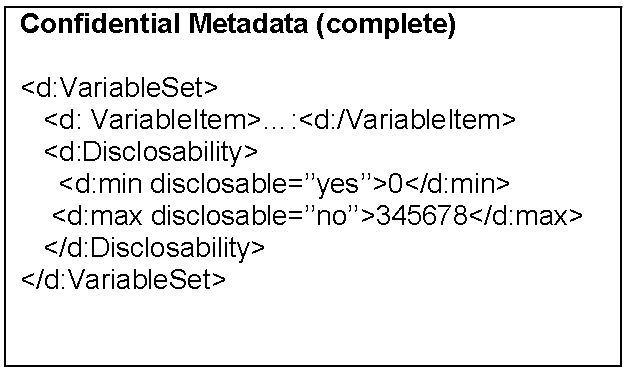
\includegraphics[width=0.4\textwidth]{ConfidentialMetadata-left}}
\only<2->{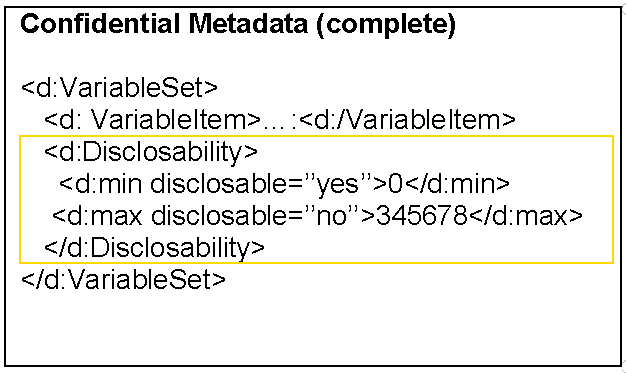
\includegraphics[width=0.4\textwidth]{ConfidentialMetadata-left-hilite}}\pause \pause &
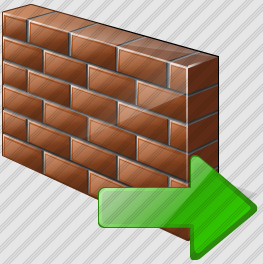
\includegraphics[width=0.1\textwidth]{wall-export-small}&
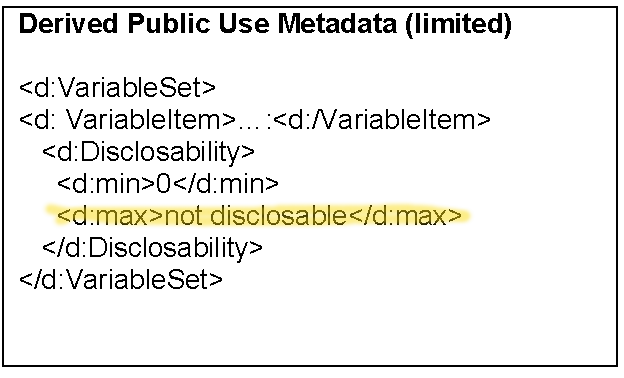
\includegraphics[width=0.4\textwidth]{ConfidentialMetadata-right}
\end{tabular}
\end{block}
\end{frame}

\begin{frame}
\frametitle{Database design}
\begin{block}{Multiple sources}
\begin{itemize}
\item Data-curator-provided metadata (possibly regularly updated, PRUNED)
\item User-provided metadata (wiki)
\item Alternate sources (IPUMS data to describe Decennial Census)
\end{itemize}
\end{block}
\begin{block}{Multiple outputs}
\begin{itemize}
\item Local query
\item Remote federation or export
\item Synchronization back to data-curator (data enclave!)
\end{itemize}
\end{block}
\end{frame}

\begin{frame}
\frametitle{Generic description}
\centering
\includegraphics[width=0.9\textwidth]{"CCBMR"}
\end{frame}

\begin{frame}[fragile]
\frametitle{Identifiers}
\begin{block}{Unique identifiers for {\it articles}}
\begin{verbatim}
Huberman, B. A.
Sociology of science:
Big data deserve a bigger audience
Nature, 2012, 482, 308-308
doi:10.1038/482308d
\end{verbatim}
\end{block}
\begin{block}{Unique identifiers for {\it data}}
``DOI names are assigned to any entity for use on digital networks. 
They are used to provide current information, including where they (or information about them) can be found on the Internet.
Information about a digital object may change over time, including where to find it, but its DOI name will not change.''
\tiny http://datacite.org/whatisdoi, accessed on Sept 26, 2012.
\end{block}

\end{frame}

\begin{frame}
\frametitle{State of the implementation}
\begin{block}{DDI extension}
Being formalized.
\end{block}
\begin{block}{DOI assignment}
Our project (NCRN) will assign DOI if not provided by curator/owner. May be validated by disclosable checksums (MD5 or similar) to verify change of files. (additional dataset-level metadata!)
\end{block}
\begin{block}{Database}
Design finalized, first connectors implemented, alpha-quality implementation with IPUMS, SIPP Synthetic Beta, simulated SIPP Gold Standard up and running.
\end{block}
\end{frame}

\subsection{Further links}
\begin{slide}
\frametitle{The end}
\begin{block}{Thank you}
\begin{itemize}
\item \cite{AbowdVilhuberBlock2012} for more details
\item \href{http://www.ilr.cornell.edu/LDI/}{Labor Dynamics Institute}
\item \href{http://www.vrdc.cornell.edu}{VirtualRDC @ Cornell}
\item \href{http://www.ncrn.cornell.edu/}{NCRN Cornell website}
\end{itemize}
\end{block}
\end{slide}

\begin{frame}[fragile]
\begin{verbatim}
$Id: Presentation-PSD-subdoc.tex 396 2013-11-03 22:29:27Z lv39 $
\end{verbatim}
\end{frame}

%%% Local Variables:
%%% mode: latex
%%% End:

\ifpdf
\embedfile{\jobname-subdoc.tex}
\fi

\part<presentation>{Appendix}

% $Id: Presentation-PSD-appendix.tex 396 2013-11-03 22:29:27Z lv39 $ 
% $URL: https://forge.cornell.edu/svn/repos/ncrn-cornell/branches/papers/PSD2012/Presentation/Presentation-PSD-appendix.tex $ 

\section{Extra slides}


\begin{frame}
\frametitle{}
\tiny
\bibliography{../abbrev,../paper}
\bibliographystyle{IEEEtranS}



\end{frame}

\ifpdf
\embedfile{\jobname-appendix.tex}
\fi

\end{document}


